


%!TEX TS-program = xelatex
%!TEX encoding = UTF-8 Unicode
%!BIB TS-program = biber
%!BIB program = biber
\documentclass[12pt,twoside]{book}
%\usepackage{extsizes}
\usepackage{geometry}                % See geometry.pdf to learn the layout options. There are lots.
\geometry{a4paper}                   % ... or a4paper or a5paper or ... 
%\geometry{landscape}                % Activate for for rotated page geometry
%\usepackage[parfill]{parskip}    % Activate to begin paragraphs with an empty line rather than an indent
\geometry{left=3cm}
\geometry{right=3cm}
\geometry{bottom=2cm}
\geometry{top=2cm}
\usepackage{graphicx}
\usepackage{amssymb}

\usepackage{polyglossia}
\usepackage[babel]{csquotes} 
\setdefaultlanguage{german}

\usepackage{titlesec}
\usepackage{hyperref}
\usepackage[all]{hypcap} % Make references jump to the figure and not to the caption.
\usepackage{enumitem}

\usepackage{wasysym}

\usepackage{booktabs}
\usepackage{tabularx}

\usepackage{todonotes}

\usepackage{float}

\usepackage{tikz}

\usepackage{ifplatform}

\usepackage{savesym}
\savesymbol{iint}
\savesymbol{iiint}
\usepackage{amsmath}

\setlength{\parindent}{0cm}
\setlength{\parskip}{\medskipamount}

% Will Robertson's fontspec.sty can be used to simplify font choices.
% To experiment, open /Applications/Font Book to examine the fonts provided on Mac OS X,
% and change "Hoefler Text" to any of these choices.

\usepackage{fontspec,xltxtra,xunicode}

\ifmacosx
	\newcommand{\romanFont}{Hoefler Text}
\else
	\newcommand{\romanFont}{Linux Libertine O}
\fi

\defaultfontfeatures{Mapping=tex-text}
\setmainfont[Mapping=tex-text]{\romanFont}
%\setsansfont[Scale=MatchLowercase,Mapping=tex-text]{Gill Sans}
%\setmonofont[Scale=MatchLowercase]{Andale Mono}

%\newcommand{\HRule}{\rule{\linewidth}{0.1pt}}
%\newcommand{\logoheight}{2.5cm}

\renewcommand{\title}{DAI Infoboard}
\renewcommand{\author}{Tom Nick}
%\date{}                                           % Activate to display a given date or no date

% PDF properties
\hypersetup{
	pdftitle={\title{}},
	pdfauthor={\author{}}
}

\usepackage[style=authoryear,natbib=true,backend=biber]{biblatex}
\bibliography{bachelorthesis}{}

\setlength{\bibitemsep}{8pt}
%\setlength{\bibhang}{0.2cm}

\usepackage{xpatch}
\xpretobibmacro{author}{\mkbibbold\bgroup}{}{}
\xapptobibmacro{author}{\egroup}{}{}
\xpretobibmacro{bbx:editor}{\mkbibbold\bgroup}{}{}
\xapptobibmacro{bbx:editor}{\egroup}{}{}

\renewcommand*{\labelnamepunct}{\mkbibbold{\addcolon\space}}


\usepackage{changepage}

\makeatletter
\renewcommand\listoffigures{%
    \section*{\listfigurename}% Used to be \section*{\listfigurename}
      \@mkboth{\MakeUppercase\listfigurename}%
              {\MakeUppercase\listfigurename}%
    \@starttoc{lof}%
    }
\makeatother

\makeatletter
\renewcommand{\todo}[2][]{\tikzexternaldisable\@todo[#1]{#2}\tikzexternalenable}
\makeatother

\setcounter{secnumdepth}{3}
\setcounter{tocdepth}{2}

%\newcommand*{\fullref}[1]{\hyperref[{#1}]{\autoref*{#1} \nameref*{#1}}}
\newcommand*{\fullref}[1]{\hyperref[{#1}]{\autoref*{#1} (\nameref*{#1})}}

\newcommand{\makemu}{{\fontspec{Linux Libertine O}μ}}

\usepackage{multirow}

\usepackage{capt-of}

\usepackage[hang,flushmargin,bottom]{footmisc} 

\newenvironment{absolutelynopagebreak}
  {\par\nobreak\vfil\penalty0\vfilneg
   \vtop\bgroup}
  {\par\xdef\tpd{\the\prevdepth}\egroup
   \prevdepth=\tpd}

\usepackage{titlesec}

\titleformat{\chapter}[display]
    {\normalfont\huge\bfseries}{\chaptertitlename\ \thechapter}{20pt}{\Huge}
\titlespacing*{\chapter}{0pt}{0pt}{40pt}

\usetikzlibrary{arrows,automata,positioning}

\usepackage{soul}

\usepackage{fancyhdr}
\fancyhead{}
\fancyfoot{}
\fancyhead[RE]{\textsc{\nouppercase{\rightmark}}}
\fancyhead[LO]{\textsc{\nouppercase{\leftmark}}}

\fancyfoot[CO,CE]{\thepage}
\pagestyle{fancy}

\setlength{\headheight}{14.5pt}

\let\cleardoublepage\clearpage

\usepackage[section]{placeins}

\usepackage{afterpage}
\newcommand\blankpage{%
    \null
    \thispagestyle{empty}%
    \addtocounter{page}{-1}%
    \newpage}



\begin{document}

% Titlepage
\begin{titlepage}
%\includegraphics[height=\logoheight,page=1]{Telekom_Logo_bw.pdf} \hfill \includegraphics[height=\logoheight,page=1]{TU_Logo.pdf}
\begin{center}
%\vspace{1cm}
%{\Huge Bachelor}\\
{\Huge \textsc{Technische Universität Berlin}}
{\fontsize{2.5cm}{2cm}\selectfont \textsc{Bachelor Thesis}\par}
\vspace{1cm}
\hrule
\vspace{0.3cm}
{\Huge \textsc{\title{}}\par}
~\\[0.1cm]
{\Large Supervisor: Prof. Albayrak}\\[0.1cm]
{\Large Advisors: -}\\[0.3cm]
{\Large Written by \author{}}\\[0.1cm]
{\Large \today}
\vspace{0.55cm}
\hrule
\end{center}
%\vspace{1cm}
\vfill
\begin{center}{\Large\textbf{Abstract}}\end{center}

Das DAI-Labor ist ein Innovationsleiter in Sachen verteiltee Suchmaschinen - welche nun nicht mehr reine Forschung sind, sondern wie deren PIA-System von vielen Verwaltungen als Alternative zu privaten Suchmaschinen benutzt wird. Einer der Kernherrausforderungen bei Suchmaschinen mit vielen komplett seperaten Suchindizes ist es die Ergebnisse dieser zusammen zu führen und für den Endbenutzer zu visualiesieren. Diese Arbeit zielt darauf ab eine Visualisierungsform die ähnlich zu einer \textit{social media wall} sein soll für diese Ergebnisse zu untersuchen und zu erstellen. Desweiteren werden kollabaritive Elemente untersucht d.h. Ergebnisse mehrerer Benutzer werden gleichzeitig angezeigt und eine Anzeige vergleichbar mit der \textit{frontpage} von reddit, wo die Suchergebnisse aller Benutzer angezeigt werden. Das Ergebnis ist eine voll funktionsfähige Webapplikation die neben der reinen Visualisierung und Interaktion der Elemente,\textit{Gamification} benutzt um die (kollabaritive) Nutzung zu fördern indem Benutzer \textit{belohnt} werden für die Benutzung sowie dafür das andere Benutzer ihre Inhalte \textit{gut} finden.

\end{titlepage}

\pagenumbering{roman}

%\blankpage

\chapter*{Declaration of authorship}

I hereby certify that the thesis I am submitting is entirely my own original work except where otherwise indicated. I am aware of the University's regulations concerning plagiarism, including those regulations concerning disciplinary actions that may result from plagiarism. Any use of the works of any other author, in any form, is properly acknowledged at their point of use.\footnote{The template for this declaration of authorship was taken from \url{https://www.wiwi.hu-berlin.de/international/mems/upload/authorship}.}

\vspace{2cm}

Berlin, \today\\
\textbf{Place, date}\hfill\textbf{Signature}

\tableofcontents
\newpage

\pagenumbering{arabic}

\chapter{Einleitung}

\section{Motivation}

Die gemeinsame Darstellung von Inhalten verschiedener Quellen ist ein interessantes und weit erforschtes Thema. Die grundsätzliche Idee ist dem Benutzer die Benutzung bzw. die Konsumierung von Inhalten angenehmer zu gestalten indem ein einheitliches Interface für Inhalte geschaffen wird. Bevor der \textit{digitalen Revolution} war dies ein immens aufwendiges und kostpieliges Unterfangen, als Beispiel sei die frühen Enzyklopädien genannt\footnote{Enzyklopädien sind insofern eine einheitliche Aggregierung des Inhalts, das sie versucht haben sämtliches Wissen in einer Quelle bereitzustellen die homogen in Sprache und Darstellung ist.}. Durch die momentan verfügbaren Technologien ist das erstellen einer einheitlichen Datenquelle für verschiedene Inhalte deutlich einfacher geworden, wobei die Schwierigkeit einer guten zusammenführung dennoch weiterhin besteht und Produkte die dies gut machen sehr erfolgreich sind - wie z.B. die Suchmaschine von Google.
Wenn man sich jedoch auf eine Teilmenge der verfügbaren Informationen beschränkt wie z.B. Nachrichten die per RSS\footnote{Ein weit verbreitetes Dateiformat im Internet \url{http://de.wikipedia.org/wiki/RSS}} verfügbar sind ist es deutlich einfacher eine angemessene zusammenführung der Inhalte zu gestalten, prominente Beispiele für eine Anwendung dieser Art ist z.B. die Nachrichten-Applikation \textit{pulse}\footnote{\url{https://www.pulse.me/}} die auf Basis von RSS ein angenehmens und sehr attraktives Interface für die gleichzeitige Konsumierung mehrerer Nachrichtenseiten anbietet, der Erfolg von \textit{pulse} spricht für sich\footnote{ca. 22 Millionen Downloads auf dem Android-System}.

Diese Arbeit zielt auf einen Spezialfall der Darstellungsformen verschiedener Inhalte ab, die der \textit{social media wall} was eine populäre Form für Inhalte mit kurzen Texten und oder Bildern ist\footnote{Natürlich sind auch Inhalte anderer Art möglich, jedoch sind die Elemente solcher Wände in jeglichem Aspekt daraufhin optimiert.}.

\section{Relevante Arbeiten}

Eine sehr gute Auflisting verschiedener \textit{social media wall}-Applikationen bietet \citep{hofram}. Die Homogenität dieser Angebote ist erstaunlich, würde man die Produkte zweier verscheidener Anbieter nebeneinander sehen wäre der größte Unterschied kleinere stylistische Unterschiede wie benutzte Farben oder ähnliches. Leider sind die wenigsten Produkte in einer Demo zu testen, da die Lösungen meistens zugeschnitten werden für den Kunden, welcher diese meistens auf großen Veranstaltungen wie Konzerten verwendet. \\

\begin{figure}[H]
    \centering
    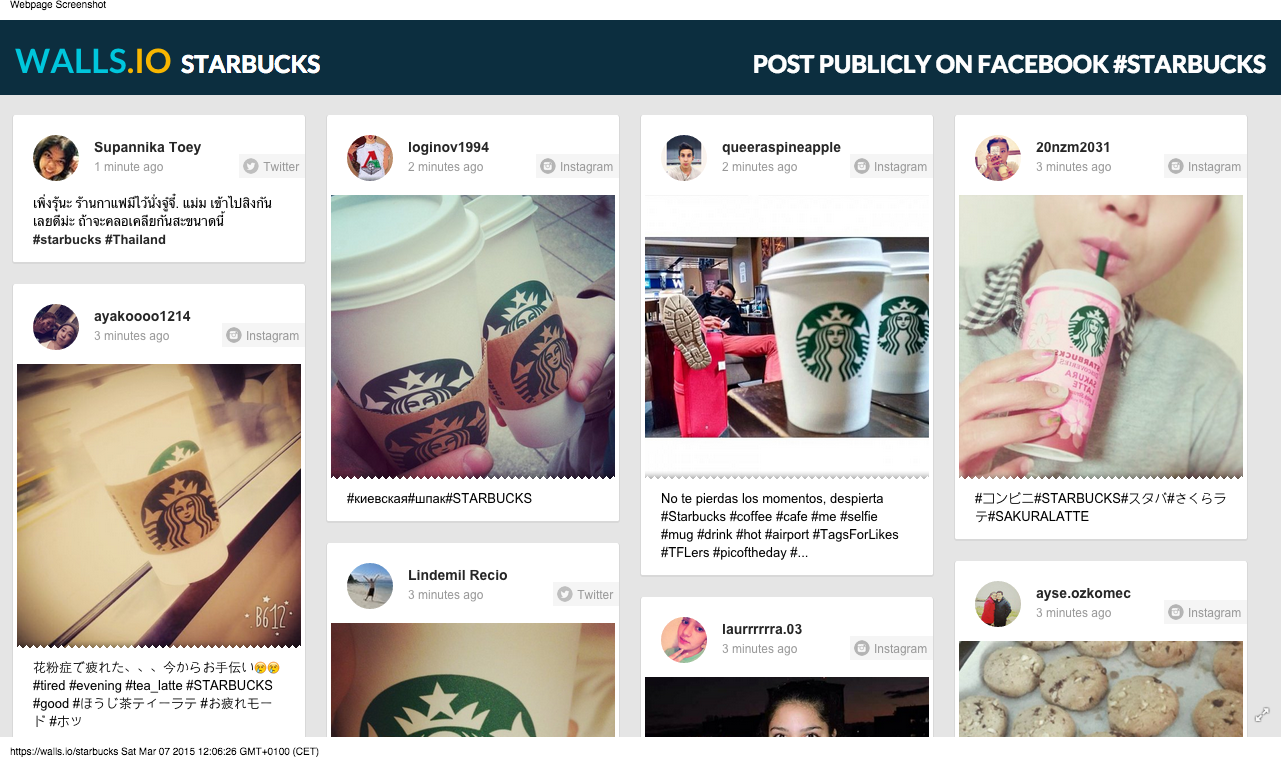
\includegraphics[width=0.8\textwidth]{images/Starbucks.png}
    \caption{Eine \textit{social media wall} vom Anbieter walls.io}
    \label{fig:awesome_image}
\end{figure}

Insofern sind diese Angebote für diese Arbeit nicht wirklich lohnenswert weiter zu analysieren und werden als grobe Inspiration für das Design benutzt.

\chapter{Umsetzung}

\section{Design}

Der wichtigste Aspekt für den Benutzer ist eine attraktive Darstellung und angenehme Bedienung der Applikation, natürlich neben dem Aspekt das es technisch an nichts mangelt d.h. es gibt keine Programmfehler und die nötigen Funktionen sind vorhanden. Im folgenden werden die einzelnen Aspekte der Darstellung dargestellt um die Findung der endgültigen Darstellung zu erklären.

\subsection{Layout}

Wie \textit{social media walls} oder Websiten wie pinterest\footnote{\url{http://pinterest.com}} oder gar Microsoft mit ihrem metro-Design es gezeigt haben ist die aktuell beste Darstellung für Medioninhalte verschiedener Art ein Layout basierend auf Kacheln. Bei dem Anordnen gibt es verschiedene Ansätze:

\begin{itemize}
  \item \textbf{Spaltenbasierte Anordnung} \\
  Bei dieser Form werden die einzelnen Datenpunkte in Form von Kacheln mit einheitlicher Breite und variabler Höhe in Spalten in der Größenordnung von 3-5 dargestellt.

  \begin{figure}[H]
    \centering
    \includegraphics[width=0.5\textwidth]{images/livewall_columns.pdf}
    \caption{Spaltenbasierte Anordnung der Inhalte}
    \label{fig:awesome_image}
  \end{figure}

  \textbf{Vorteile} \\
  Die Vorteile liegen in der Simplizität der Implementierung und der Intuivität des \textit{content-flows} d.h. neuer Inhalt wird oben eingefügt und alter rutscht nach unten, wobei jeweils nur eine Spalte \textit{verrutscht} je neuem Datenpunkt.
  Weiterhin ermöglicht die Variable Höhe viel Flexibilität bei dem Anzeigen des Inhalts - z.B. könnten lange Texte angemessen gut angezeigt werden ohne die Zeichenanzahl zu limitieren oder ähnliches.

  \textbf{Nachteile}\\
  Der Größteile Nachteil ist die starre des Layouts, da alle Objekte die gleiche Breite haben ist man stark limitiert wie man die Inhalte darstellt.

  \item \textbf{Rasterbasierte Anordnung}
  Bei dieser Form werden die einzelnen Datenpunkte in einem einheitlichen Raster dargestellet, d.h. die darstellende Fläche wird in einem Raster der Größe $(a, b)$ unterteilt, die Kacheln können nun die Größe $(x, y)$ mit $ x \in \{1, \dots, a, y \in 1, \dots, b$ besitzen.

  \begin{figure}[H]
    \centering
    \includegraphics[width=0.8\textwidth]{images/livewall_grid.pdf}
    \caption{links: Das Raster des Grids, rechts: eine zufällige Benutzung des Grids}
    \label{fig:awesome_image}
  \end{figure}
  
  \textbf{Vorteile} \\
  \begin{itemize}
    \item Ansprechendes Aussehen
    \item Wichtigkeit kann durch größe der Kachel dargestellt werden
    \item Unterschiede in der Darstellung gleicher Datenpunkte durch unterschiedliche Größe
    \item Vorteilhaft bei der Anzeige ohne Interaktion, da es keine abgeschnittenen Inhalte gibt wie bei dem Spaltendesign
  \end{itemize}

  \textbf{Nachteile}\\
  \begin{itemize}
    \item komplexes flow-Verhalten bei neuem Inhalt
    \item Es müssen komplexere Methoden benutzt werden um Löcher zu verhindern
    \item Es müssen Design für die verschiedenen Kachelgrößen erstellt werden
    \item unterschiedliche Darstellungsformen können unübersichtlich wirken
  \end{itemize}

\end{itemize}





\chapter{Technische Umsetzung}

\section{Wahl der Technologie}

Die Wahl der zu verwendeten Technologie ist ein wichtiger Punkt der die darauffolgende Entwicklung und spätere Wartung beeinflusst. Es wird versucht auf folgende Punkte einzugehen:

\begin{itemize}
  \item Technologie ist \textit{erwachsen} \\
  Die verwendete Bibilothek oder ähnliches ist nicht Brandneu und hat sich in vielen Applikationen bewährt, sie ist soweit ausgereift das workarounds oder bugfixes nur in den seltensten Fällen nötig sein sollten.
  \item Die Technologie hat keine große Einstiegsbarriere \\
  Es wird versucht nicht allzu viele Frameworks zu benutzen und wenn, dann welche die weitesgehend bekannt sind und oder in dem DAI-Labor viel benutzt werden. Wenn Bibliotheken verwendet werden, wird darauf geachtet das sie einfach zu lernen sind und intuitiv in der Benutzung.
  \item Die Technologie ist zukunftsicher \\
  Es ist immer schwer ab zu schätzen welche Technologie länger überleben wird, doch wird versucht anhand von Faktoren wie Popularität, Aktivität der Entwicklung und Einsatz bei großen Firmen dies so gut wie möglich zu garantieren.
\end{itemize}

\subsection{Frontend}

Eine sehr gepflegte Liste der derzeit verfügbaren Technologien im Bereich Frontend ist verfügbar auf github\footnote{https://github.com/dypsilon/frontend-dev-bookmarks}.

Für das Frontend ist erstmal die Frage zu klären ob ein Framework a la AngularJs oder EmberJS verwendet werden soll. Dagegen spricht wie oben schon gennante die initiale Lernkurve, was es schwer machen könnte das System einfach wartbar zu machen, auch stellen Frameworks oft bei Applikationen die etwas ausgefeilteres machen als die breite Masse ein Problem da, da die Abstraktion des Frameworks oft etwas verbirgt was benötigt wird.

Ein großer Faktor der in anderen Umgebungen lange Zeit keine Rolle mehr spielt ist die größe des Quelltextes der verwendeten Bibliotheken/Frameworks. Bevor bei Javascript irgendeine Bibliothek benutzt werden kann muss sie zuerst beim Benutzer heruntergeladen und ausgeführt werden, was bei langsamen Computern mit nicht perfekter Internetverbindung ein enormer Bestandteil ist. Um den Punkt nochmal zu verdeutlichen wurde ein kleiner Test gemacht. Dazu wurde eine Ember-Demoapplikation ausgeführt\footnote{Auf einem Macbook Air mid 2013 in minimal Konfiguration und dem Chrome Browser in Version 41, die vorhandene Internetverbindung hatte eine Übertragungsrate von $50000 \frac{\text{bit}}{s}$} die sehr wenig \textit{business-logic} besitzt, sodass sehr gut zu zeigen ist wieviel das herunterladen und ausführen nur der Bibliotheken ausmachen.
Die Anwendung ist auf github zu finden\footnote{\url{http://jkneb.github.io/ember-crud/unstyled/\#/users}}.
\begin{figure}[H]
    \centering
    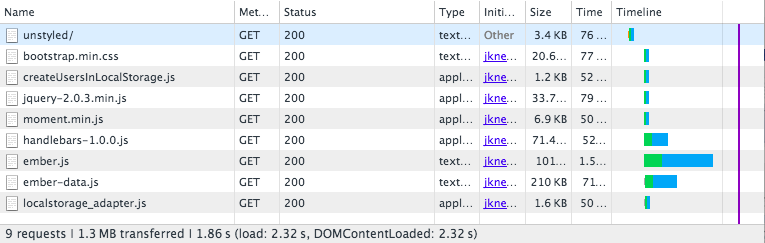
\includegraphics[width=0.8\textwidth]{images/performance_1.png}
    \caption{Übertragungszeit der benötigten Dateien}
    \label{fig:awesome_image}
\end{figure}
\begin{figure}[H]
    \centering
    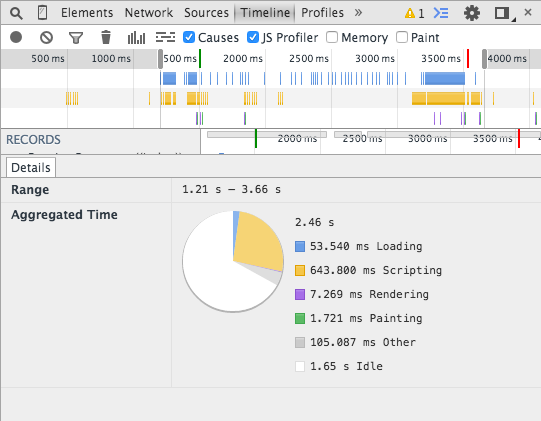
\includegraphics[width=0.6\textwidth]{images/performance_2.png}
    \caption{Benötigte Ausführungszeit der Skriptdatein}
    \label{fig:awesome_image}
\end{figure}
Die Ergebnisse zeigen, dass ganze $1.86s$ zum Übertragen und etwa $600ms$ zum ausführen den Anwendung benötigt wurden.




\subsection{Backend}

% One of the key-difficulties is the problem of 

\chapter{Andere Arbeiten}


\chapter{Ausblick}

\chapter{Appendix}

\cleardoublepage
\phantomsection

\printbibliography

\cleardoublepage
\phantomsection

\end{document}  



